\documentclass{beamer}

% \usepackage[]{geometry}
% \usepackage[utf8]{inputenc} % Needs to be loaded before csquotes
\usepackage[english]{babel}
\usepackage{csquotes,xpatch} % Needs to be loaded after babel
\usepackage[style=authoryear]{biblatex}
\addbibresource{../bibliography.bib}

% \usepackage{algorithm}
% \usepackage{algpseudocode}
\usepackage{amsmath,amssymb,amsbsy,amsthm}
\usepackage{bm}
\usepackage{graphicx}
% \usepackage{hyperref}
% \usepackage{mathptmx} %Times new romans text
% \usepackage{My_AMA}
\usepackage{pgfplots}
\pgfplotsset{compat=1.18}

\usepackage{soul}
\usepackage{subcaption}
\usepackage{tikz}
% \usetikzlibrary{arrows.meta,backgrounds}
\graphicspath{ {../images} }

% \usepackage{unicode-math}

\usepackage{xcolor}
\definecolor{ruby}{RGB}{192, 47, 29}

%%%% CUSTOM COMMANDS %%%%%
\DeclareMathOperator*{\argmax}{arg\,max}
\DeclareMathOperator*{\argmin}{arg\,min}
\DeclareMathOperator{\cov}{cov}
\DeclareMathOperator{\E}{\mathbb{E}}
\DeclareMathOperator{\Exp}{Exp}
\DeclareMathOperator{\MVN}{MVN}
\newcommand{\N}{\mathcal{N}}
\DeclareMathOperator{\p}{\mathbb{P}}
\DeclareMathOperator{\Pois}{Pois}
\newcommand{\R}{\mathbb{R}}

\newtheorem{definnn}{Definition}

\makeatletter
\providecommand*{\diff}%
    {\@ifnextchar^{\DIfF}{\DIfF^{}}}
\def\DIfF^#1{%
    \mathop{\mathrm{\mathstrut d}}%
        \nolimits^{#1}\gobblespace}
\def\gobblespace{%
        \futurelet\diffarg\opspace}
\def\opspace{%
        \let\DiffSpace\!%
        \ifx\diffarg(%
            \let\DiffSpace\relax
        \else
            \ifx\diffarg[%
               \let\DiffSpace\relax
            \else
               \ifx\diffarg\{%
                   \let\DiffSpace\relax
               \fi\fi\fi\DiffSpace}


%Information to be included in the title page:
\title{Efficient Likelihood Approximation via Gaussian Processes}
\subtitle{With an Application to a \emph{P. Vivax} Malaria Model}
\author{Jacob Cumming}
\institute{University of Melbourne, Walter and Eliza Hall Institute}
\date{June 2024}
\logo{%
  \makebox[0.95\paperwidth]{%
  
\includegraphics[height=1cm,keepaspectratio]{unimelb_logo.png}%
  \hfill%
  
\includegraphics[height=1cm,keepaspectratio]{WEHI_RGB_logo.png}%
}
}
% \logo{
\includegraphics[height=1cm]{unimelb_logo}}
% \logo{
\includegraphics[height=1cm]{WEHI_RGB_logo}}

\begin{document}

\frame{\titlepage}

% Why is Vivax of interest? More complicated than \emph{P. falciparum} since it
% has a

\begin{frame}
    \frametitle{Introduction and Motivation}
    \begin{itemize}
        \item 600,000 deaths/year, 75\% children under 5
        \item Two main species \emph{P. vivax} and \emph{P. falciparum}
        \item \emph{P. falciparum} main cause of death, but
              \emph{P. vivax} historically underestimated.
        \item Proportion of \emph{P. vivax} cases increased over last 50 years.
    \end{itemize}
\end{frame}

\begin{frame}
    \frametitle{\emph{P. vivax} has Dormant Stage}
    \begin{figure}
        \centering
        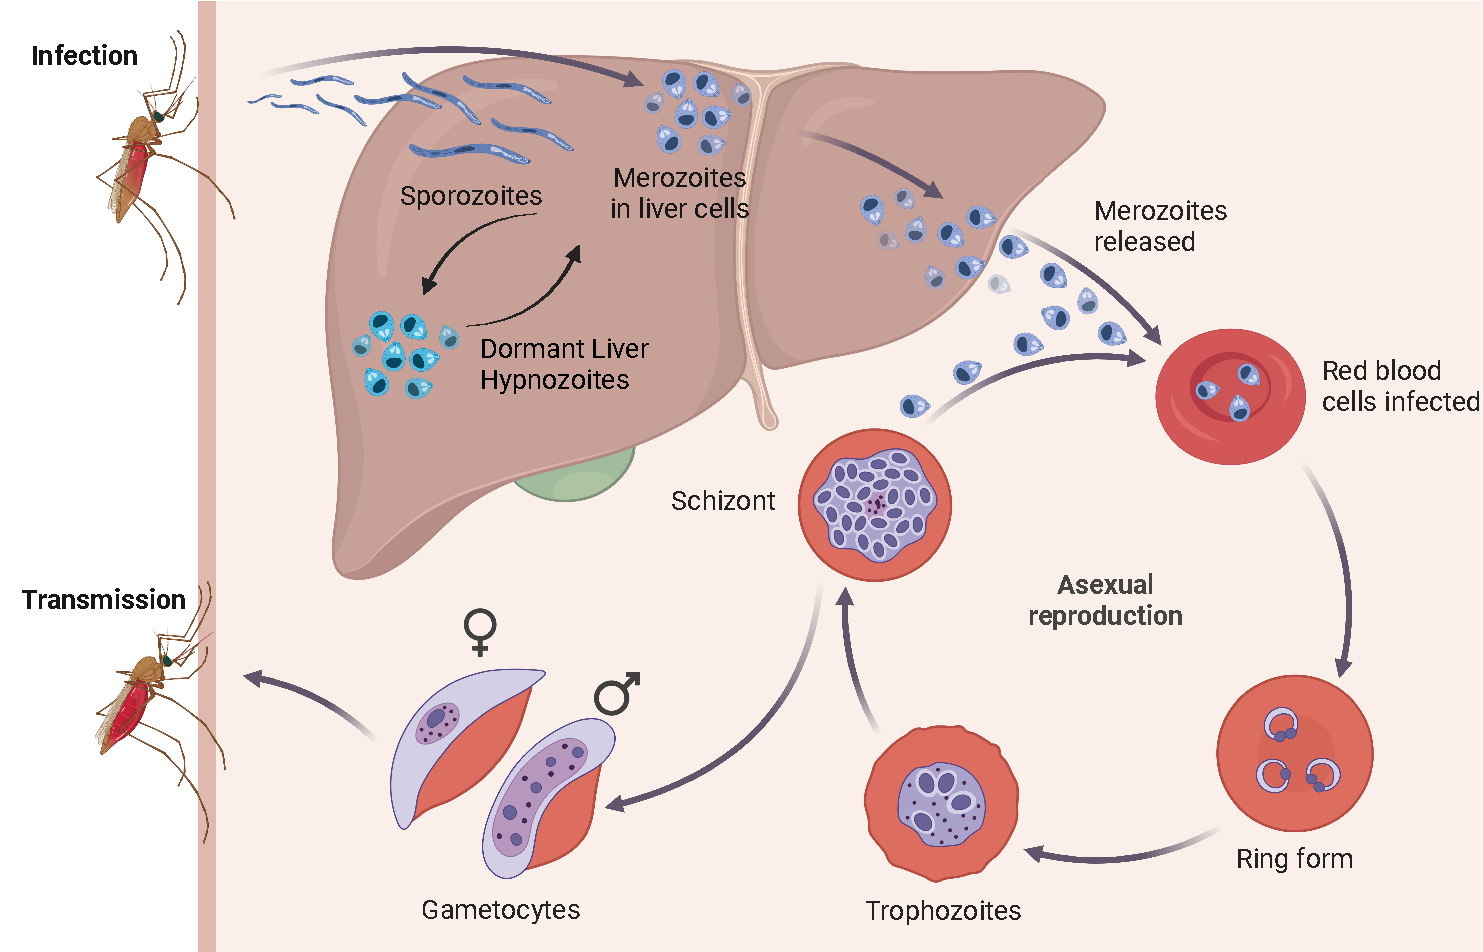
\includegraphics[width=0.8\textwidth]{vivax_lifecycle_full.pdf}
        \caption{\emph{P. vivax} lifecycle. Created with BioRender.com}
    \end{figure}
\end{frame}

\begin{frame}
    \frametitle{Vivax Model - Champagne et.\ al}
    \begin{figure}[htbp]
        \centering
        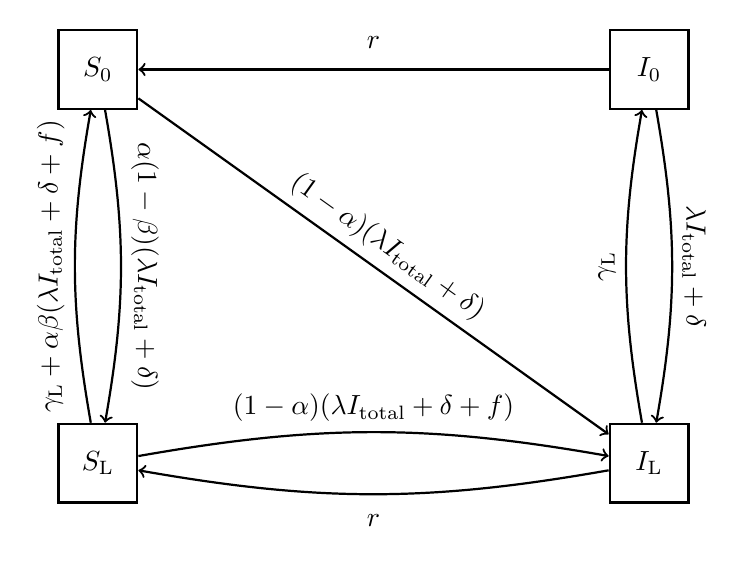
\begin{tikzpicture}[thick]
            \node[draw, minimum size=1cm] (S0) {$S_0$};
            \node[draw, right of=S0, minimum size=1cm, node distance=7cm] (I0)
            {$I_0$};
            \node[draw, below of=S0, minimum size=1cm, node distance=5cm] (SL)
            {$S_\mathrm{L}$};
            \node[draw, below of=I0, minimum size=1cm, node distance=5cm] (IL)
            {$I_\mathrm{L}$};
            \draw[->] (S0) edge[sloped] node[above]
                {$(1 - \alpha)(\lambda I_\mathrm{total} + \delta)$} (IL);
            \draw[->] (S0) edge[in = 80, out = 280, sloped] node[above]
                {$\alpha( 1 -\beta)(\lambda I_\mathrm{total} + \delta)$} (SL);
            \draw[->] (SL) edge[in = 260, out = 100, sloped] node [above]
                {
                    $
                        \gamma_\mathrm{L}
                        + \alpha\beta(\lambda I_\mathrm{total} + \delta + f)
                    $
                } (S0);
            \draw[->] (SL) edge[in = 170, out = 10, sloped] node [above]
                {$(1 -\alpha)(\lambda I_\mathrm{total} + \delta + f)$} (IL);
            \draw[->] (IL) edge[in = -10, out = 190] node [midway, label=below:
            {$r$}] (r) {} (SL);
            \draw[->] (IL) edge[in = 260, out = 100, sloped] node [above]
                {$\gamma_\mathrm{L}$} (I0);
            \draw[->] (I0) edge[in = 80, out = 280, sloped] node [above]
                {$\lambda I_\mathrm{total} + \delta$} (IL);
            \draw[->] (I0) edge node [midway, label=above:{$r$}] (r2) {} (S0);
        \end{tikzpicture}
        \caption{\cite{champagne_using_2022} \textit{P.\ vivax} model}
    \end{figure}
\end{frame}

\begin{frame}
    \frametitle{Champagne Model Parameters}\begin{itemize}
        \item $\alpha:$ proportion of those infected who clear blood stage
              infections through treatment
        \item $\beta:$ proportion of those cleared of blood stage infection
              who are also cleared of liver
              stage parasites
              (radical cure)
        \item $\lambda:$  rate of infection
        \item $\gamma_L:$ rate of liver stage disease clearance
        \item $f:$ rate of relapse
        \item $r:$ rate of blood stage clearance
        \item $\delta = 0$ importation rate (fixed)
    \end{itemize}
\end{frame}

% \begin{frame}
%     \frametitle{Ordinary Differential Equations - Champagne et.\ al}
%     \begin{align*}
%         \frac{\diff I_\mathrm{L}}{\diff t}
%         = & (1 - \alpha)(\lambda I_\mathrm{total} + \delta)(S_0 + S_\mathrm{L})
%         + (\lambda I_\mathrm{total} + \delta)I_0                                        \\
%           & + (1 - \alpha)fS_\mathrm{L} - \gamma_\mathrm{L}I_\mathrm{L}
%         - rI_\mathrm{L}                                                                 \\
%         \frac{\diff I_0}{\diff t}
%         = & -(\lambda I_\mathrm{total} + \delta)I_0
%         + \gamma_\mathrm{L}I_\mathrm{L} - rI_0                                          \\
%         \frac{\diff S_\mathrm{L}}{\diff t}
%         = & -(1 - \alpha(1 - \beta))(\lambda I_\mathrm{total} + \delta + f)S_\mathrm{L} \\
%           & + \alpha(1-\beta)(\lambda I_\mathrm{total} + \delta)S_0
%         - \gamma_\mathrm{L}S_\mathrm{L} + rI_\mathrm{L}                                 \\
%         \frac{\diff S_0}{\diff t}
%         = & -(1 - \alpha\beta)(\lambda I_\mathrm{total} + \delta)S_0
%         + (\lambda I_\mathrm{total} + \delta)\alpha\beta S_\mathrm{L}                   \\
%           & + \alpha\beta fS_\mathrm{L} + \gamma_\mathrm{L}S_\mathrm{L} + rI_0
%     \end{align*}
% \end{frame}

% Even with improved techniques (tau leaping)
\begin{frame}
    \frametitle{The Problem}
    \begin{itemize}
        \item How to calibrate model parameters?
        \item <2-> Simulations take long time (and models get a lot more
              complicated)
    \end{itemize}
\end{frame}

\begin{frame}
    \frametitle{Notation}
    \begin{itemize}
        \item $\bm{\theta}$ vector of parameters
              - e.g.\ $[\alpha, \beta, \gamma_L, \lambda, f, r]^T$
        \item $\mathbf{Y}_\text{obs}:$ a (summary) vector of observed data
              e.g.\ (weekly) incidence, prevalence, (monthly) hospitalisations
              % \item <2-> Model $f:\bm{\Theta} \to \bm{\mathcal{Y}}.$
              %       \begin{itemize}
              %           \item $\bm{\Theta}:$ parameter space
              %           \item $\bm{\mathcal{Y}}:$ model output space
              %       \end{itemize}
        \item <2->$\mathbf{Y}_{\bm{\theta}}:$ a random vector
              of model statistics for given $\bm{\theta}.$
    \end{itemize}
\end{frame}

\begin{frame}
    \frametitle{In an ideal world...}
    \begin{itemize}
        \item There would be an explicit form for the likelihood:
              $$
                  \mathcal{L}(\bm{\theta})
                  := \Pr(
                  \mathbf{Y}_{\bm{\theta}} = \mathbf{Y}_\text{obs}
                  | \bm{\theta}
                  )
              $$
        \item $\hat{\bm{\theta}}
                  = \argmax_{\bm{\theta}} \mathcal{L}(\bm{\theta})$
        \item $\Pr(\bm{\theta}|\mathbf{Y}_\text{obs})
                  \propto \mathcal{L}(\bm{\theta})\Pr(\bm{\theta})$
        \item Off to the pub
    \end{itemize}
\end{frame}

\begin{frame}
    \frametitle{Or not...}
    \begin{itemize}
        \item Explicit likelihoods often don't exist/are intractible
              \begin{itemize}
                  \item Champagne model
                  \item Agent based models.
              \end{itemize}
    \end{itemize}
\end{frame}

\begin{frame}
    \frametitle{A Standard Bayesian Solution}
    \begin{itemize}
        \item Approximate Bayesian Computation (ABC)\begin{enumerate}
                  \item Sample $\bm{\theta}_i$ from prior
                  \item Run model and observe $\mathbf{Y}_{\bm{\theta}_i}$
                  \item Accept or reject $\bm{\theta}_i$ run based on how well
                        $\mathbf{Y}_{\bm{\theta}_i}$ `matches' $\mathbf{Y}_\text{obs}.$
              \end{enumerate}
    \end{itemize}
\end{frame}

\begin{frame}
    \frametitle{What is `matches'?}
    \begin{enumerate}
        \item $\mathbf{Y}_{\bm{\theta}_i} = \mathbf{Y}_\text{obs}$
              \begin{itemize}
                  \item <2-> Good luck...
              \end{itemize}
        \item <3-> Rescale $\mathbf{Y}$s, and use discrepency function
              $D:\R^d\times\R^d\to\R$ e.g.\ $p$-norm
              $$
                  D(\mathbf{Y}_{\bm{\theta}_i}, \mathbf{Y}_\text{obs})
                  :=\left(\sum_{j = 1}^d
                  \left|\{\mathbf{Y}_{\bm{\theta}_i}\}_j
                  - \{\mathbf{Y}_\text{obs}\}_j\right|^p\right)^{1/p}
              $$
    \end{enumerate}
\end{frame}

\begin{frame}
    \frametitle{Discrepency Function}

    $\mathcal{D}(\bm{\theta})
        := D(\mathbf{Y}_{\bm{\theta}}, \mathbf{Y}_\text{obs})$ how `close' our
    model is to the observed data using parameters $\bm{\theta}$

\end{frame}

\begin{frame}
    \frametitle{ABC}
    \begin{enumerate}
        \item Sample $\bm{\theta}_i$ from prior
        \item Run model
        \item Accept $\bm{\theta}_i$ if $\mathcal{D}(\bm{\theta}_i) < \varepsilon.$
    \end{enumerate}
\end{frame}

% \begin{frame}
%     \frametitle{Uniform Acceptance Probability}
%     \begin{figure}
%         \centering
%         \begin{tikzpicture}
%             \begin{axis}[
%                     xlabel={$\mathcal{D}_(\bm{\theta})$},
%                     ylabel={Probability of Acceptance},
%                     xmin=0, xmax=2,
%                     ymin=0, ymax=1.1,
%                     axis lines=left,
%                     xtick={0.5},  % Define custom x tick at x = epsilon
%                     xticklabels={$\varepsilon$},  % Label the custom tick as epsilon
%                     % grid=major,
%                 ]

%                 % Plot y = 1 for 0 < x < epsilon
%                 \draw[blue!50!black, thick] (0,1) -- (0.5,1);

%                 % Plot y = 0 for x >= epsilon
%                 \draw[blue!50!black, very thick] (0.5,0) -- (2,0);

%                 % Mark epsilon
%                 \draw[dashed] (0.5,0) -- (0.5,1);

%             \end{axis}
%         \end{tikzpicture}
%     \end{figure}
% \end{frame}

% \begin{frame}{Acceptance Probability}
%     \begin{figure}
%         \centering
%         \begin{tikzpicture}
%             \begin{axis}[
%                     xlabel={$D(S(\mathbf{Y}), S(\mathbf{Y}_\text{obs}))$},
%                     ylabel={Synthetic Likelihood},
%                     xmin=0, xmax=4,
%                     ymin=0, ymax=1.1,
%                     domain=0:4,
%                     samples=100,
%                     axis lines=left,
%                     grid=major,
%                 ]

%                 \addplot [blue!50!black, thick] {exp(-x^2/2)};

%             \end{axis}
%         \end{tikzpicture}
%     \end{figure}
% \end{frame}

\begin{frame}
    \frametitle{Overall Idea of my Research}
    \begin{itemize}
        \item ABC fixes one problem but leaves another:
              \begin{itemize}
                  \item Don't need $\mathcal{L}(\bm{\theta}).$
                  \item Evaluating $\mathcal{D}(\bm{\theta})$ takes as long as
                        a model run.
              \end{itemize}
        \item <2-> $\mathcal{D}(\bm{\theta}), \mathcal{D}(\bm{\theta}^\prime)$
              will be highly correlated when $\bm{\theta}$ is near
              $\bm{\theta}^\prime.$
              \begin{itemize}
                  \item Gaussian Processes
              \end{itemize}
    \end{itemize}
\end{frame}

\begin{frame}
    \frametitle{Gaussian Process Setup}

    Formally we can assume that
    $$\mathrm{Cov}(\mathcal{D}(\bm{\theta}_i), \mathcal{D}(\bm{\theta}_j))
        = k(\bm{\theta}_i, \bm{\theta}_j)$$ for some
    covariance kernel $k$ that decays to 0 as $\bm{\theta}_i$ is further away
    than $\bm{\theta}_j.$
\end{frame}

% \begin{frame}
%     \frametitle{Gaussian Processes}
%     \begin{itemize}
%         \item Random functions.
%         \item Common examples - Brownian motion, Ornstein Uhlenbeck process.
%     \end{itemize}
% \end{frame}

\begin{frame}
    \frametitle{Gaussian Processes on $\R^d$}
    \begin{definnn}[Gaussian Process]
        A collection of random variables $\{f\,(\mathbf{x})\}_{\mathbf{x}\in\R^d}$
        is a \emph{Gaussian process} if all finite dimensional distributions are
        multivariate normal distributed.
    \end{definnn}
    \begin{figure}
        \centering
        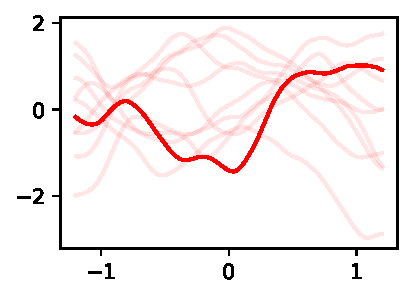
\includegraphics{maternfivehalves_kernel.pdf}
    \end{figure}
\end{frame}

% \begin{frame}
%     \frametitle{Equivalent GP definition}
%     \begin{definnn}[Gaussian Process]
%         A collection of random variables $\{f\,(\mathbf{x})\}_{\mathbf{x}\in\R^d}$
%         is a \emph{Gaussian process} if there is a function
%         $m:\mathcal{\mathbf{x}}\to\R$ and covariance kernel
%         $k:\mathcal{Y}\times\mathcal{Y}\to \R$
%         such that for all $\{\mathbf{x}_1, \mathbf{x}_2, \dots, \mathbf{x}_n\},$
%         $$\begin{bmatrix}
%                 f\,(\mathbf{x}_1) \\ f\,(\mathbf{x}_2)\\ \vdots\\ f\,(\mathbf{x}_n)
%             \end{bmatrix} \sim
%             \MVN\left(\begin{bmatrix}
%                 m(\mathbf{x}_1) \\ m(\mathbf{x}_2)\\ \vdots\\ m(\mathbf{x}_n)
%             \end{bmatrix},\, \mathbf{K}\right)$$
%         where $\mathbf{K}_{ij} := k(\mathbf{x}_i, \mathbf{x}_j).$
%     \end{definnn}
% \end{frame}

% \begin{frame}
%     \frametitle{$k$ Determines Smoothness}
%     \begin{figure}
%         \centering
%         \begin{subfigure}[t]{0.4\textwidth}
%             \centering
%             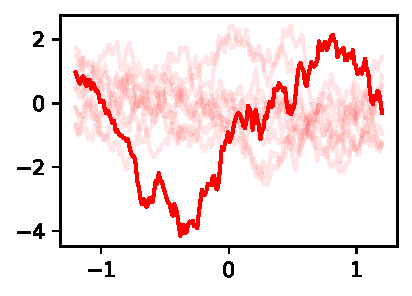
\includegraphics[width=\textwidth]{maternonehalf_kernel.pdf}
%         \end{subfigure}%
%         \begin{subfigure}[t]{0.4\textwidth}
%             \centering
%             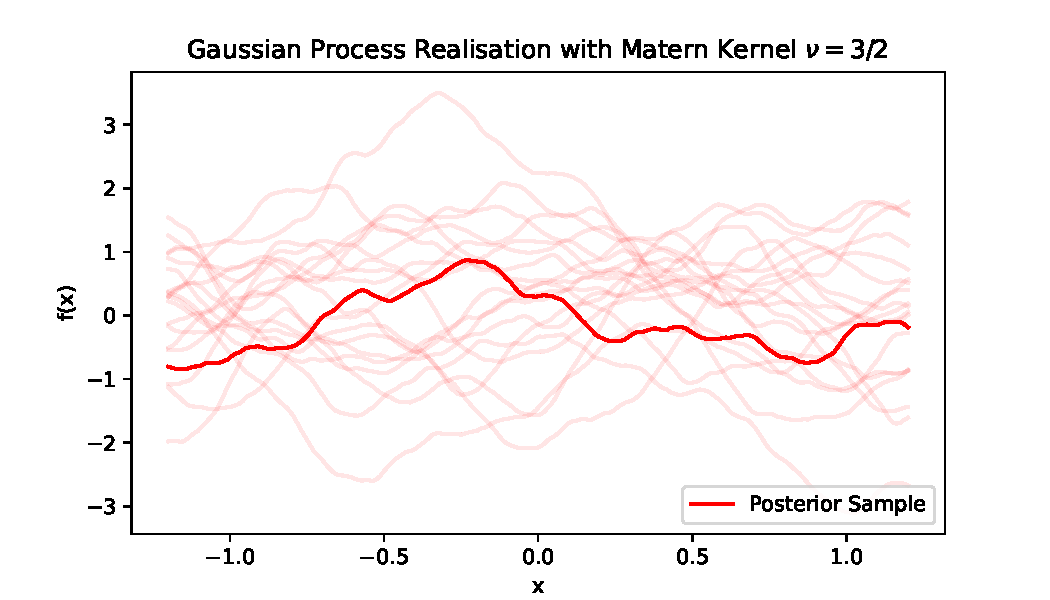
\includegraphics[width=\textwidth]{maternthreehalves_kernel.pdf}
%         \end{subfigure}
%         \begin{subfigure}[t]{0.4\textwidth}
%             \centering
%             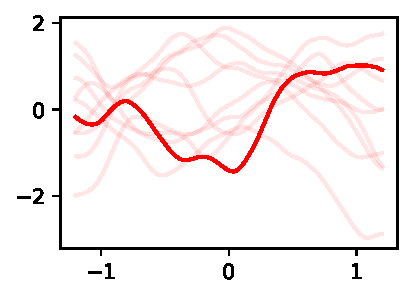
\includegraphics[width=\textwidth]{maternfivehalves_kernel.pdf}
%         \end{subfigure}%
%         \begin{subfigure}[t]{0.4\textwidth}
%             \centering
%             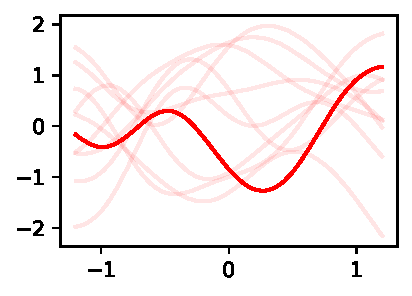
\includegraphics[width=\textwidth]{exponentiated_kernel.pdf}
%         \end{subfigure}%
%         \caption{
%             Mat\'ern 1/2, 3/2, 5/2, and squared exponential kernels.
%         }
%     \end{figure}
% \end{frame}

\begin{frame}
    \frametitle{Gaussian Process Continuity}
    \begin{itemize}
        \item Induce continuity by forcing
              $k(\mathbf{x}, \mathbf{x}^\prime) \to \mathrm{Var}(f\,(\mathbf{x}))$
              (hence $\mathrm{Cor}(f\,(\mathbf{x}), f\,(\mathbf{x}^\prime)) \to 1$)
              as $\mathbf{x}\to \mathbf{x}^\prime.$
    \end{itemize}
\end{frame}

\begin{frame}
    \frametitle{Common Covariance Kernels}
    \begin{itemize}
        \item Choice of kernel determines smoothness
        \item Mat\'ern Kernel with hyperparameter $\nu:$
              $\lfloor{\nu}\rfloor$ times mean square differentiable.
        \item $\nu\to\infty:$ infinitely mean square differentiable squared
              exponential covariance kernel (strong assumption)
              $$
                  k(x, x^\prime)
                  = \sigma^2_k\exp(-\frac{||x - x^\prime||^2}{2\ell^2})
              $$
    \end{itemize}
\end{frame}

\begin{frame}
    \frametitle{$k$ Determines Class of Functions}
    \begin{figure}
        \centering
        \begin{subfigure}[t]{0.4\textwidth}
            \centering
            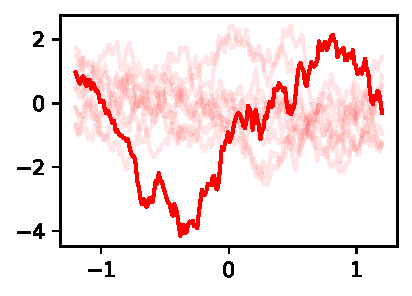
\includegraphics[width=\textwidth]{maternonehalf_kernel.pdf}
        \end{subfigure}%
        \begin{subfigure}[t]{0.4\textwidth}
            \centering
            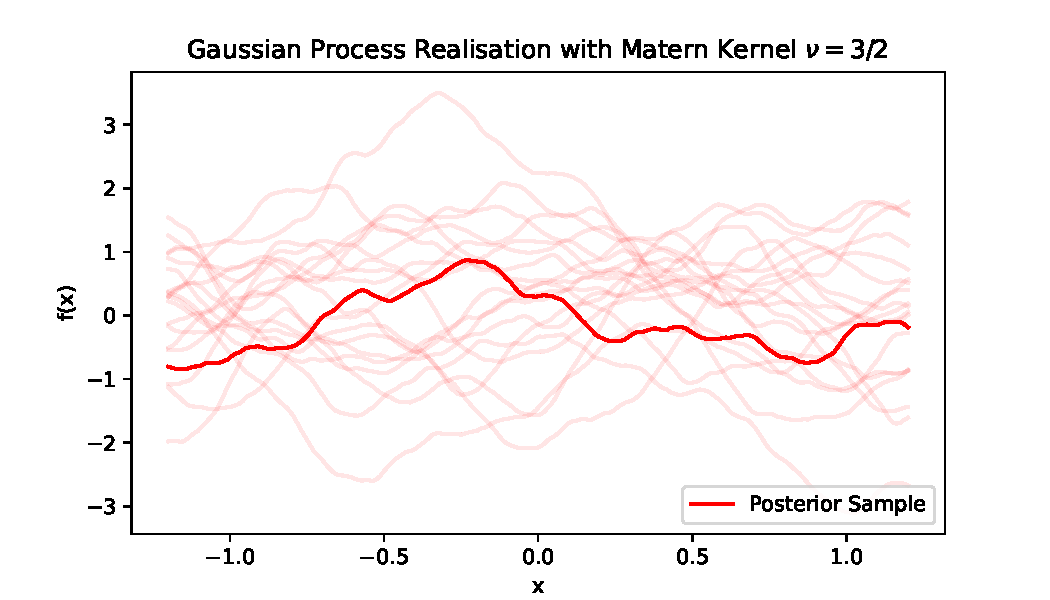
\includegraphics[width=\textwidth]{maternthreehalves_kernel.pdf}
        \end{subfigure}
        \begin{subfigure}[t]{0.4\textwidth}
            \centering
            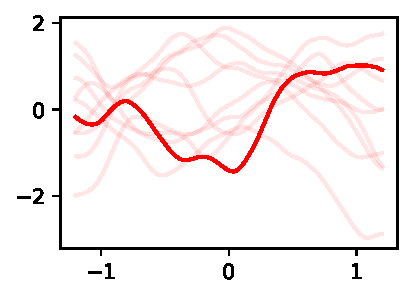
\includegraphics[width=\textwidth]{maternfivehalves_kernel.pdf}
        \end{subfigure}%
        \begin{subfigure}[t]{0.4\textwidth}
            \centering
            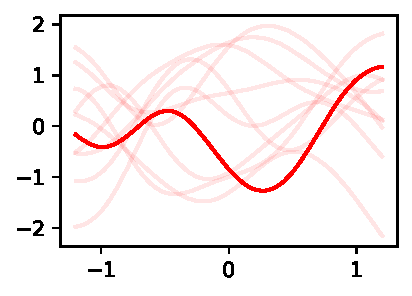
\includegraphics[width=\textwidth]{exponentiated_kernel.pdf}
        \end{subfigure}%
        \caption{
            Mat\'ern 1/2, 3/2, 5/2, and squared exponential kernels.
        }
    \end{figure}
\end{frame}

\begin{frame}
    \frametitle{Kernel Hyperparameters}
    \begin{itemize}
        \item Mat\'ern and squared exponential kernel can both be written in the
              form $k(\mathbf{x}, \mathbf{x}^\prime)
                  = \sigma_k^2\kappa(||\mathbf{x}, \mathbf{x}^\prime||/\ell)$
        \item $1/\ell$ rate of covariance decay
        \item $\sigma_k^2 = \mathrm{Var}(f\,(\mathbf{x}))$
    \end{itemize}
\end{frame}

% \begin{frame}
%     \frametitle{Kernel Hyperparameters}
%     \begin{figure}[htbp]
%         \centering
%         \begin{subfigure}[b]{0.4\textwidth}
%             \centering
%             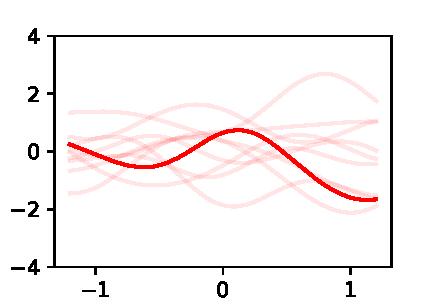
\includegraphics[width=\textwidth]{GP_ell_5_sigma2_5_tenths.pdf}
%             \subcaption{$\ell = 1/2 \quad \sigma^2_k = 1/2$}
%             \label{fig:half_half}
%         \end{subfigure}%
%         % \hfill%
%         \begin{subfigure}[b]{0.4\textwidth}
%             \centering
%             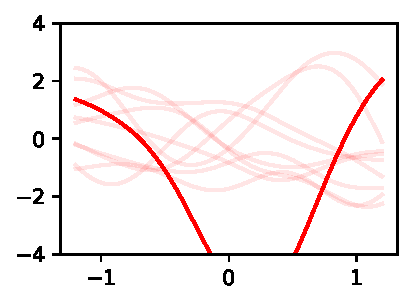
\includegraphics[width=\textwidth]{GP_ell_5_sigma2_20_tenths.pdf}
%             \subcaption{$\ell = 1/2 \quad \sigma^2_k = 2$}
%             \label{fig:half_two}
%         \end{subfigure}
%         \begin{subfigure}[b]{0.4\textwidth}
%             \centering
%             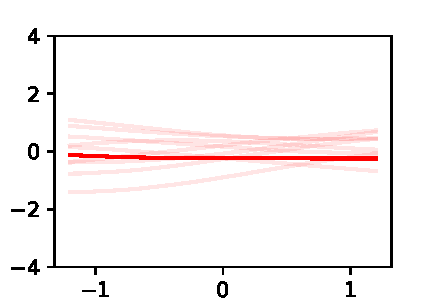
\includegraphics[width=\textwidth]{GP_ell_20_sigma2_5_tenths.pdf}
%             \subcaption{$\ell = 2 \quad \sigma^2_k = 1/2$}
%             \label{fig:two_half}
%         \end{subfigure}%
%         % \hfill%
%         \begin{subfigure}[b]{0.4\textwidth}
%             \centering
%             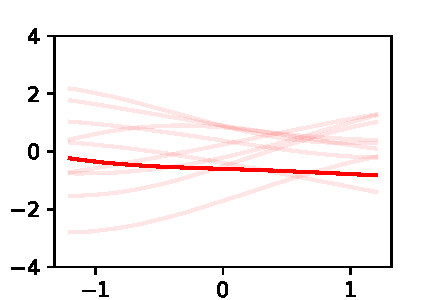
\includegraphics[width=\textwidth]{GP_ell_20_sigma2_20_tenths.pdf}
%             \subcaption{$\ell = 2 \quad \sigma^2_k = 2$}
%             \label{fig:two_two}
%         \end{subfigure}
%     \end{figure}
% \end{frame}

\begin{frame}
    \frametitle{Discrepency Function Context}
    \begin{itemize}
        \item Long term play: replace $\mathcal{D}(\bm{\theta})$ with a
              Gaussian process surrogate model approximation.
        \item <2-> What if we have observations already?
    \end{itemize}

\end{frame}

\begin{frame}
    \frametitle{Gaussian Process Regression}

    $$
        \begin{bmatrix}
            f\,(\mathbf{x}) \\
            f\,(\mathbf{x}_*)
        \end{bmatrix} \sim \MVN\left(
        \begin{bmatrix}
                m(\mathbf{x}) \\
                m(\mathbf{x}_*)
            \end{bmatrix}, \begin{bmatrix}
                K       & K_{*}  \\
                K_{*}^T & K_{**}
            \end{bmatrix}
        \right)
    $$ implies
    $$
        f\,(\mathbf{x}) | f\,(\mathbf{x}_*)
        \sim \MVN\left(
        m(\mathbf{x}) + K_{*}K_{**}^{-1}(f\,(\mathbf{x}_*) - m(\mathbf{x}_*)), \,\,
        K - K_{*}K_{**}^{-1}K_{*}^T
        \right).
    $$
\end{frame}

% \begin{frame}
%     \frametitle{Conditioning Gaussian Processes}
%     \begin{figure}
%         \centering
%         \begin{subfigure}[t]{0.4\textwidth}
%             \centering
%             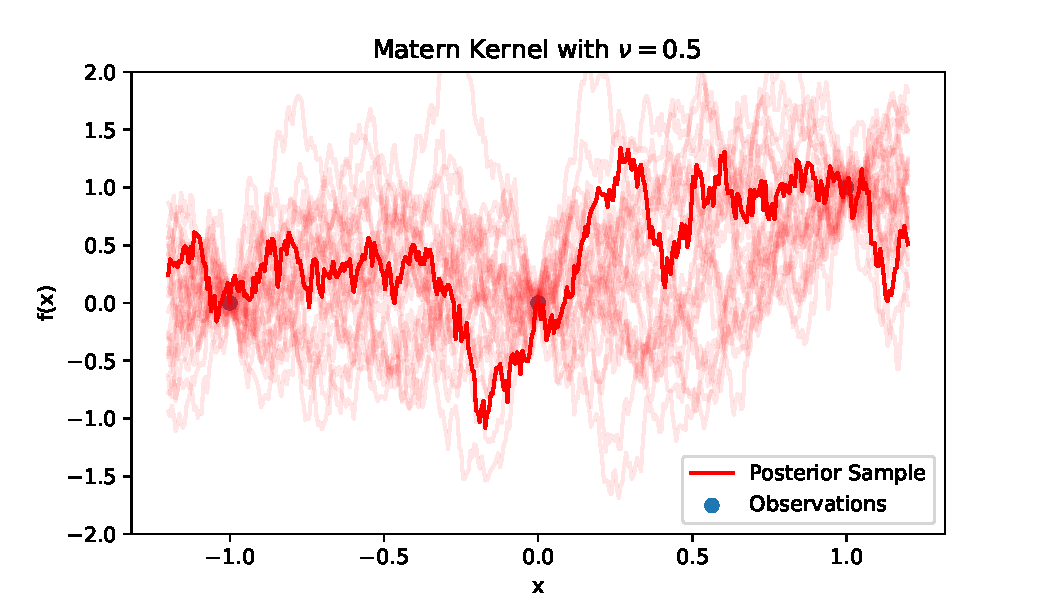
\includegraphics[width=\textwidth]{flatish_GP_matern_5.0_tenths.pdf}
%         \end{subfigure}%
%         \begin{subfigure}[t]{0.4\textwidth}
%             \centering
%             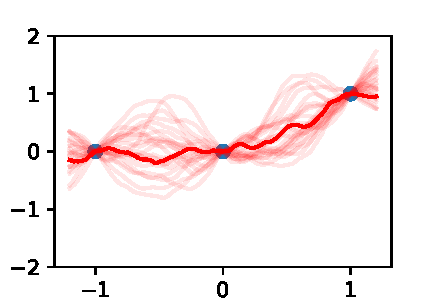
\includegraphics[width=\textwidth]{flatish_GP_matern_15.0_tenths.pdf}
%         \end{subfigure}
%         \begin{subfigure}[t]{0.4\textwidth}
%             \centering
%             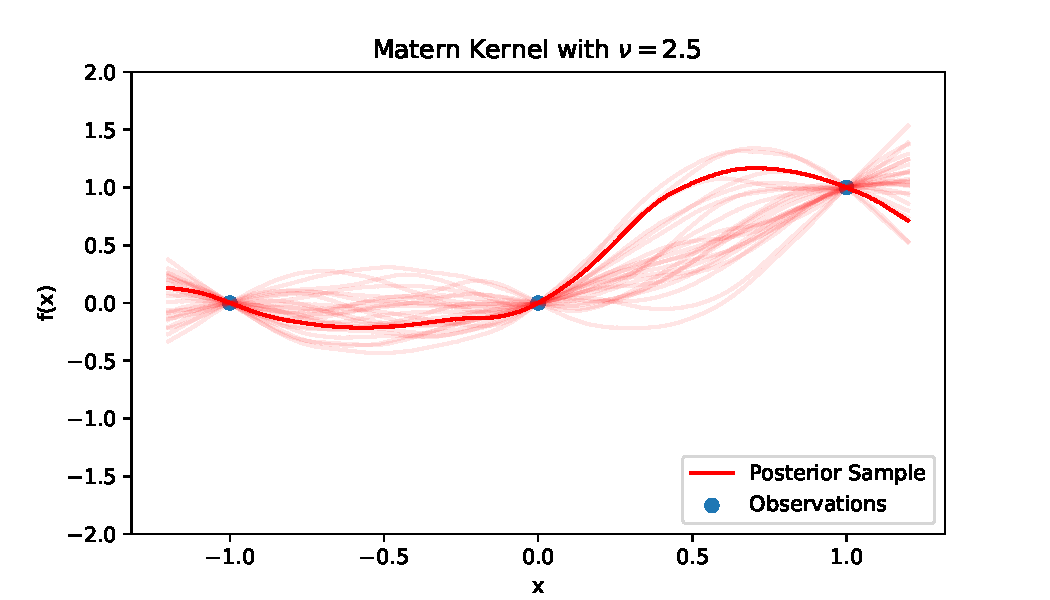
\includegraphics[width=\textwidth]{flatish_GP_matern_25.0_tenths.pdf}
%         \end{subfigure}%
%         \begin{subfigure}[t]{0.4\textwidth}
%             \centering
%             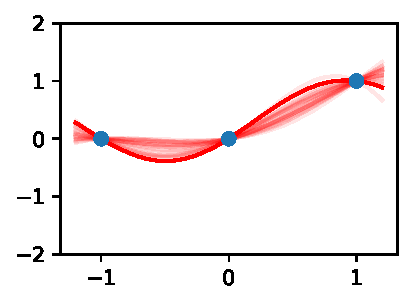
\includegraphics[width=\textwidth]{flatish_GP_ell_10_tenths.pdf}
%         \end{subfigure}%
%     \end{figure}
% \end{frame}

% \begin{frame}
%     \only<2>{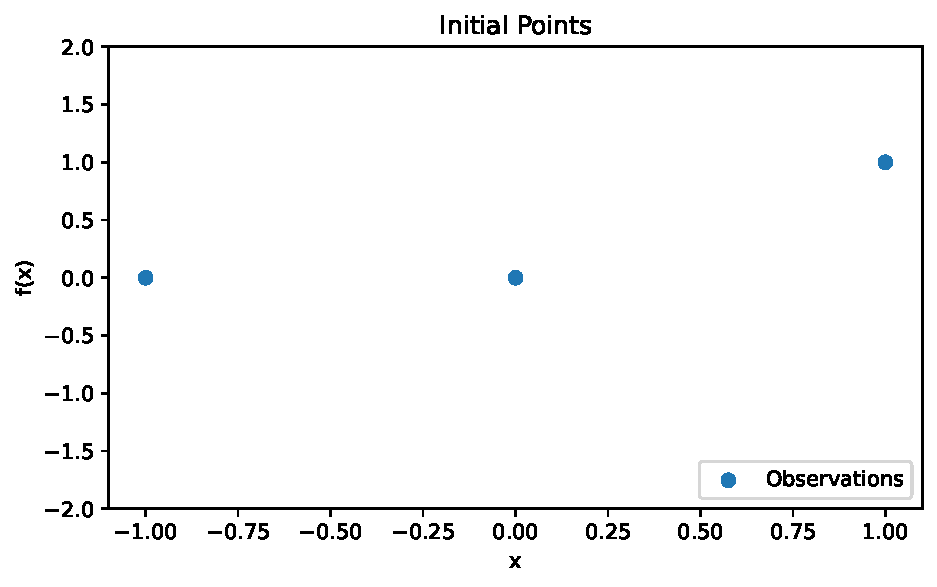
\includegraphics[width=\textwidth]{flatish_GP_bare.pdf}}
%     \only<3>{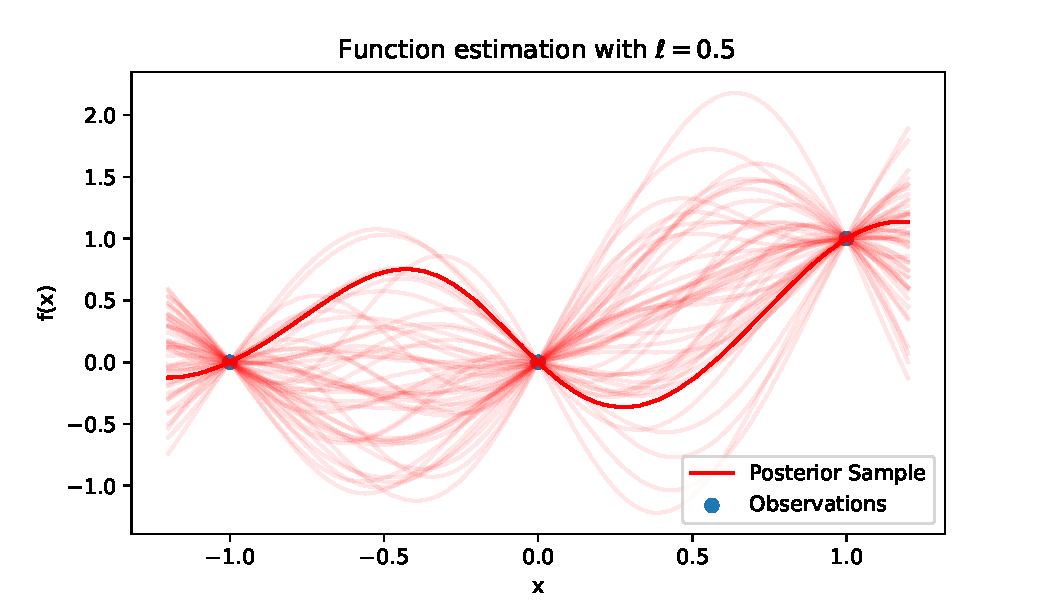
\includegraphics[width=\textwidth]{flatish_GP_ell_5_tenths.pdf}}
%     % \only<4>{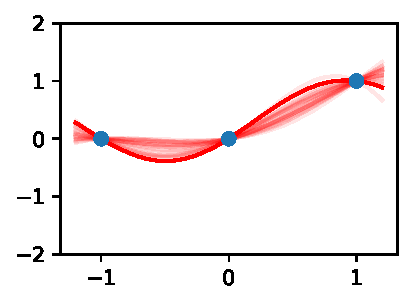
\includegraphics[width=\textwidth]{flatish_GP_ell_10_tenths.pdf}}
%     % \only<5>{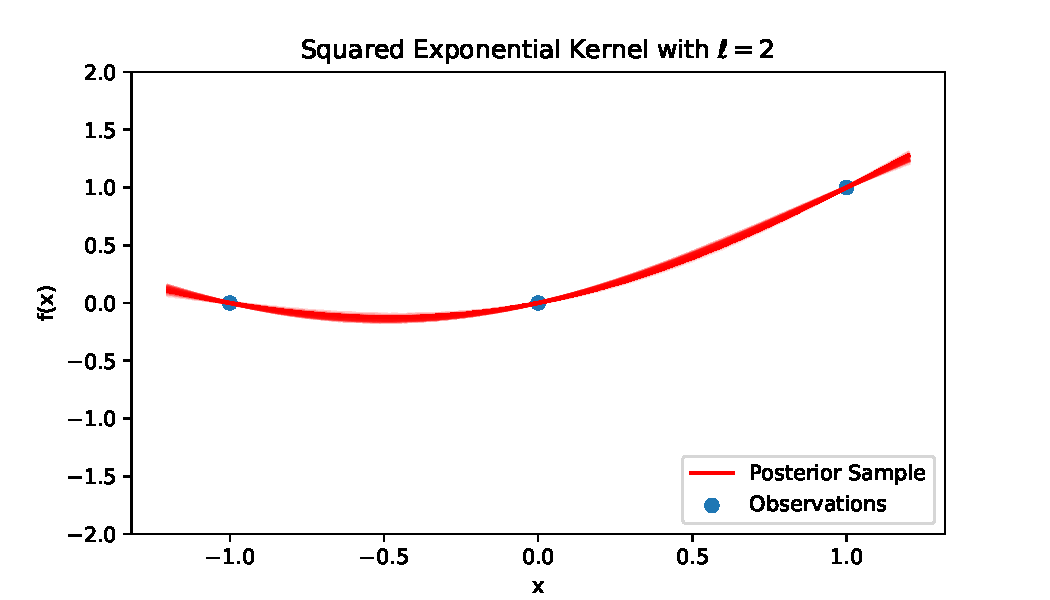
\includegraphics[width=\textwidth]{flatish_GP_ell_20_tenths.pdf}}
%     \only<6>{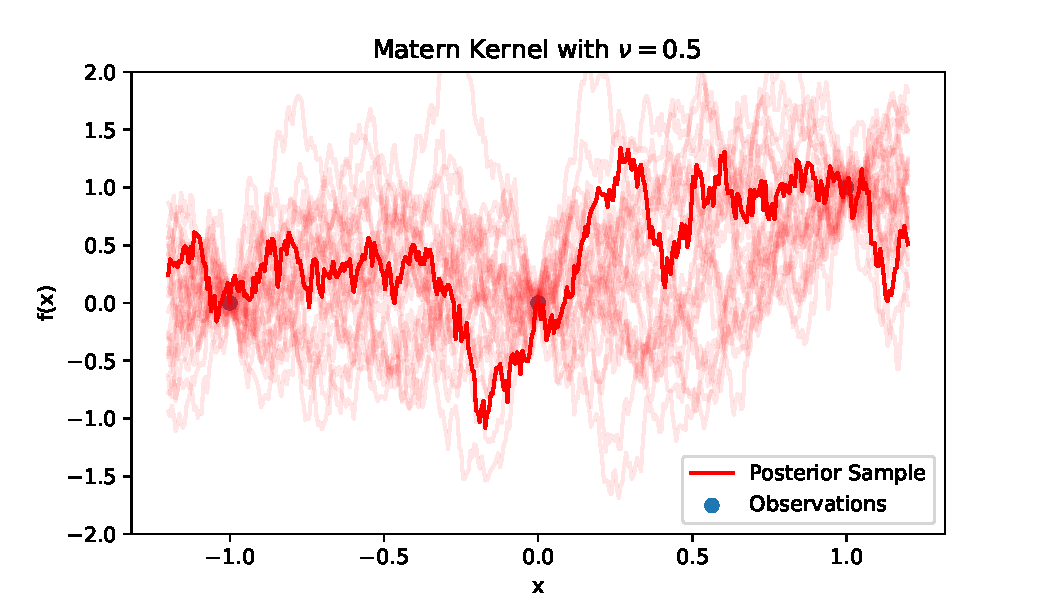
\includegraphics[width=\textwidth]{flatish_GP_matern_5.0_tenths.pdf}}
%     % \only<7>{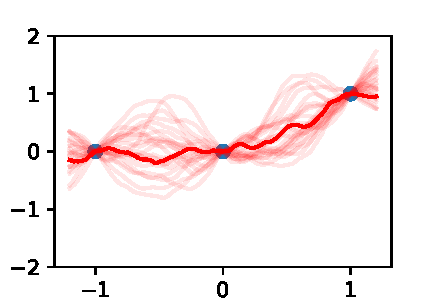
\includegraphics[width=\textwidth]{flatish_GP_matern_15.0_tenths.pdf}}
%     \only<8>{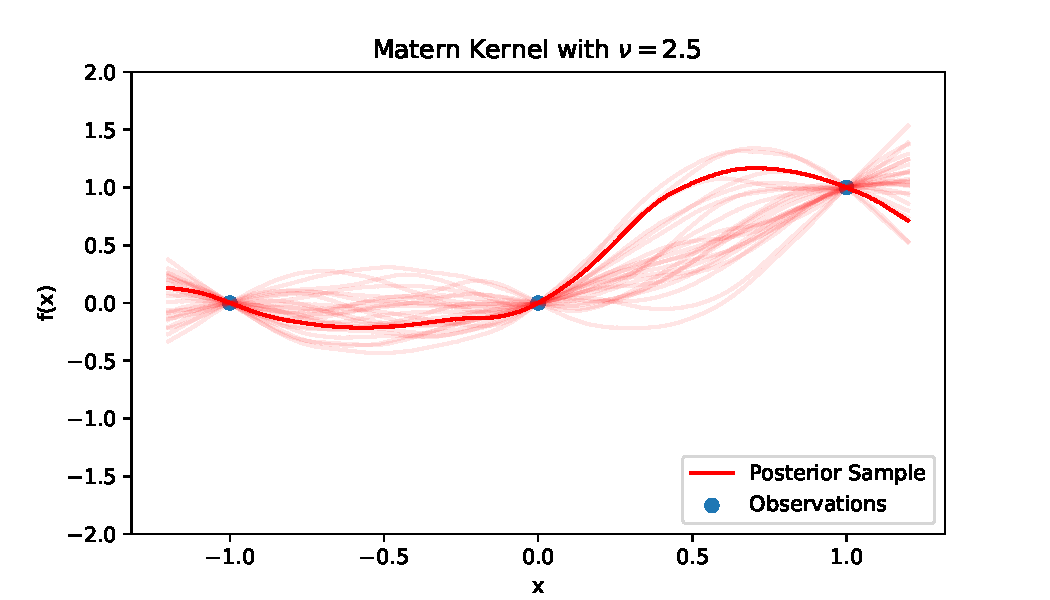
\includegraphics[width=\textwidth]{flatish_GP_matern_25.0_tenths.pdf}}
% \end{frame}

\begin{frame}
    \frametitle{GP regression on $x(x-1)(x+1)$}
    \begin{figure}
        \centering
        \begin{subfigure}[t]{0.4\textwidth}
            \centering
            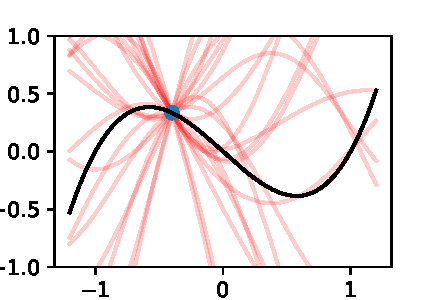
\includegraphics[width=\textwidth]{cub_GP_1_iters.pdf}
        \end{subfigure}%
        \begin{subfigure}[t]{0.4\textwidth}
            \centering
            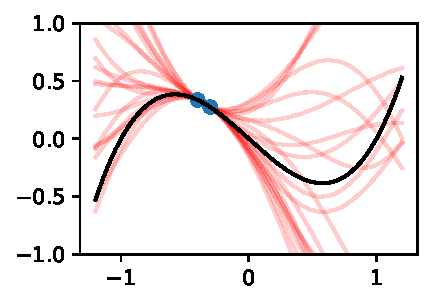
\includegraphics[width=\textwidth]{cub_GP_2_iters.pdf}
        \end{subfigure}
        \begin{subfigure}[t]{0.4\textwidth}
            \centering
            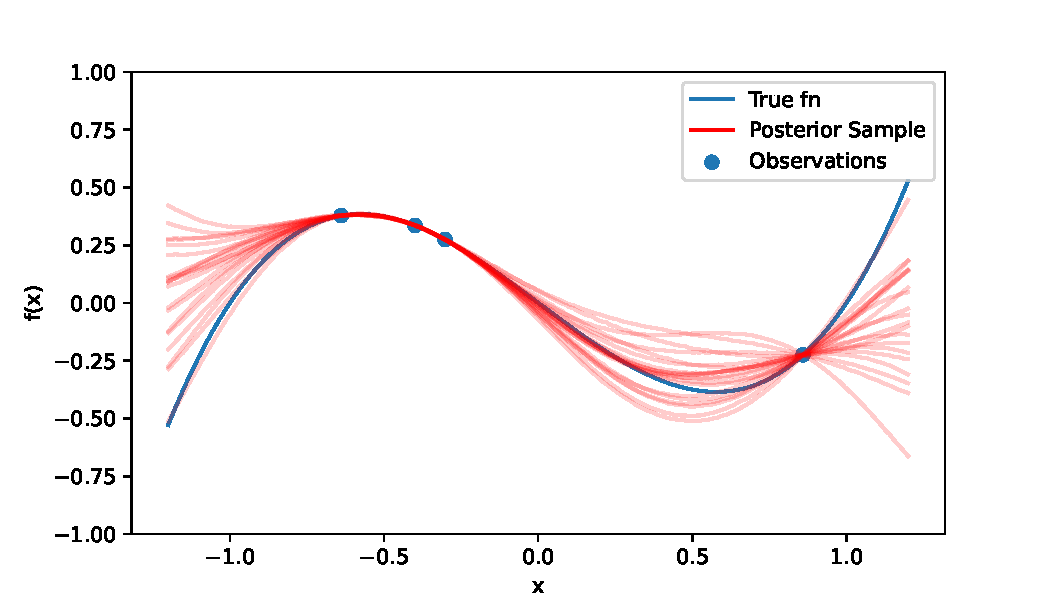
\includegraphics[width=\textwidth]{cub_GP_4_iters.pdf}
        \end{subfigure}%
        \begin{subfigure}[t]{0.4\textwidth}
            \centering
            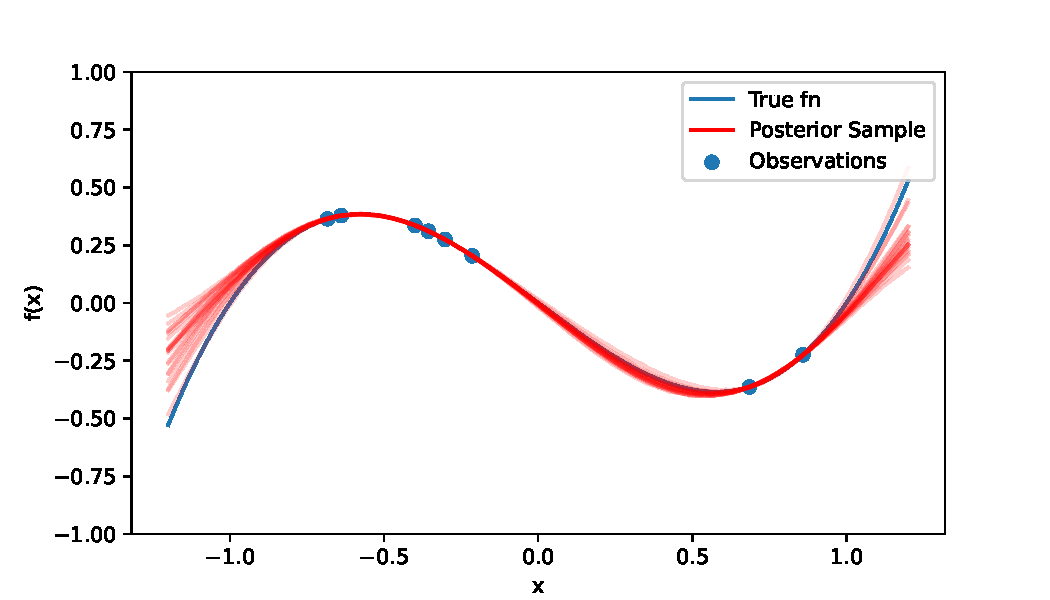
\includegraphics[width=\textwidth]{cub_GP_8_iters.pdf}
        \end{subfigure}%
    \end{figure}
\end{frame}

\begin{frame}
    \frametitle{Normal observation noise}
    If observations actually $f(\mathbf{x}_i) + \varepsilon_i,$ with
    $\varepsilon_i \sim N(0, \sigma^2_o)$ i.i.d., then
    $$
        \begin{bmatrix}
            f\,(\mathbf{x}_1) + \varepsilon_1 \\
            \vdots                            \\
            f\,(\mathbf{x}_n) + \varepsilon_n
        \end{bmatrix} \sim
        \MVN\left(\begin{bmatrix}
            m(\mathbf{x}_1) \\ \vdots\\ m(\mathbf{x}_n)
        \end{bmatrix},\, \mathbf{K} + \sigma^2_o\mathbf{I}_n\right)$$
\end{frame}

\begin{frame}
    \frametitle{
        GP regression on $x(x-1)(x+1) + \varepsilon,$
        $\varepsilon \sim N(0, \sigma^2_o)$
    }
    \begin{figure}
        \centering
        \begin{subfigure}[t]{0.4\textwidth}
            \centering
            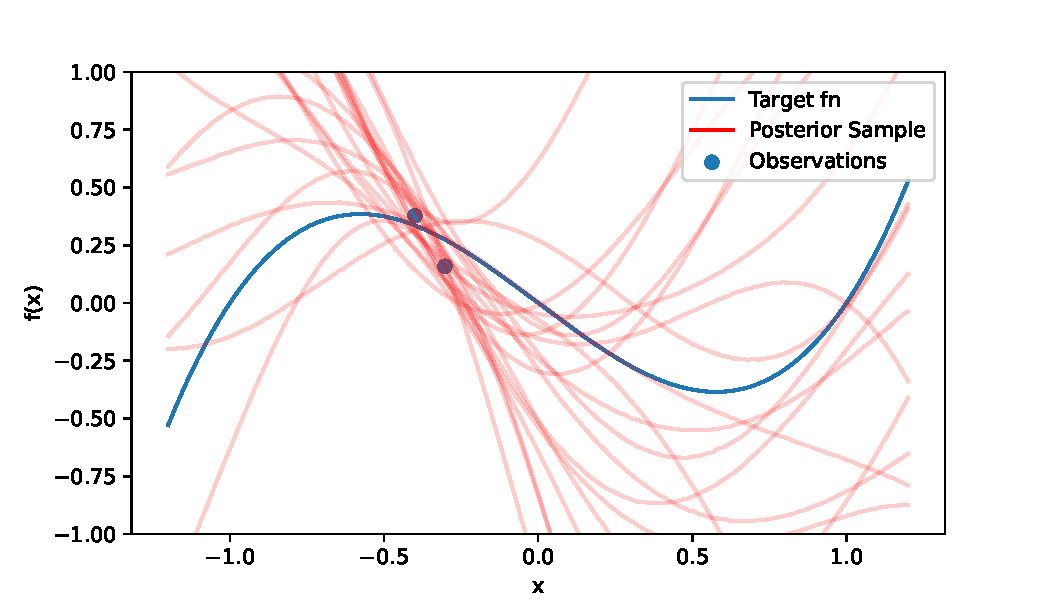
\includegraphics[width=\textwidth]{cub_GP_err_2_iters.pdf}
        \end{subfigure}%
        \begin{subfigure}[t]{0.4\textwidth}
            \centering
            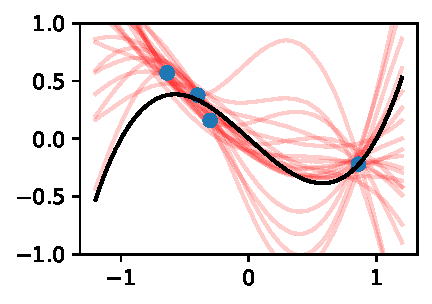
\includegraphics[width=\textwidth]{cub_GP_err_4_iters.pdf}
        \end{subfigure}
        \begin{subfigure}[t]{0.4\textwidth}
            \centering
            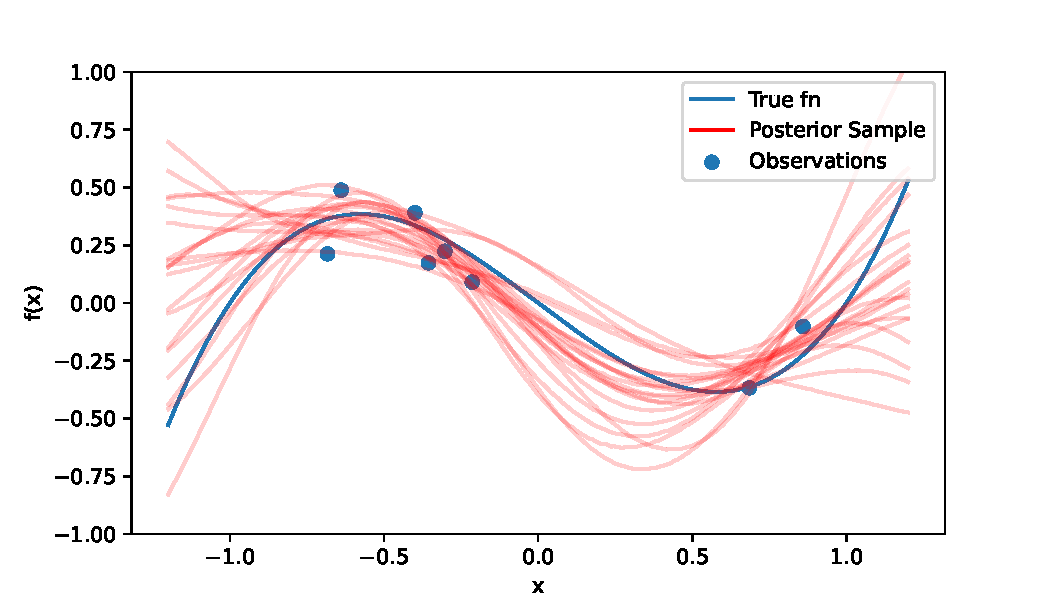
\includegraphics[width=\textwidth]{cub_GP_err_8_iters.pdf}
        \end{subfigure}%
        \begin{subfigure}[t]{0.4\textwidth}
            \centering
            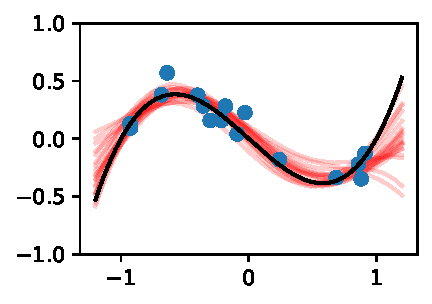
\includegraphics[width=\textwidth]{cub_GP_err_16_iters.pdf}
        \end{subfigure}%
    \end{figure}
\end{frame}

\begin{frame}
    \frametitle{Key Idea}
    \begin{itemize}
        \item If $\E[\mathcal{D}(\bm{\theta})]$ can be well approximated by a
              Gaussian process and ...
        \item <2-> $\mathcal{D}(\bm{\theta})$ approximately distributed
              $N(\E[\mathcal{D}(\bm{\theta})], \sigma^2_o)$ then...
        \item <3-> Approximate $\mathcal{D}(\bm{\theta})$ with
              $\mathcal{D}_\mathcal{GP}(\bm{\theta}),$ a Gaussian process with
              observation noise.
    \end{itemize}
\end{frame}

\begin{frame}
    \frametitle{ABC}
    \begin{enumerate}
        \item Sample $\bm{\theta}_i$ from prior
        \item Run model
        \item Accept $\bm{\theta}_i$ if
              $\mathcal{D}(\bm{\theta}_i) < \varepsilon.$
    \end{enumerate}
\end{frame}

\begin{frame}
    \frametitle{Approximate ABC...??}
    \begin{enumerate}
        \item Sample $\bm{\theta}_i$ from prior
        \item \st{Run model}
              Simulate
              $\mathcal{D}_\mathcal{GP}(\bm{\theta}_i)
                  \overset{d}{\approx}\mathcal{D}(\bm{\theta}_i) $
        \item Accept $\bm{\theta}_i$ if
              \underline{
                  $\mathcal{D}_\mathcal{GP}(\bm{\theta}_i) < \varepsilon.$
              }
    \end{enumerate}
\end{frame}

\begin{frame}
    \frametitle{Synthetic Likelihood}

    $\Pr$ drawing and accepting $\bm{\theta}$ using
    `approximate' ABC is
    $$
        \Pr(\mathcal{D}_{\mathcal{GP}}(\bm{\theta}) < \varepsilon)
        \Pr(\bm{\theta})
    $$
    and hence
    $$
        \hat{L}(\bm\theta)
        := \Pr(\mathcal{D}_{\mathcal{GP}}(\bm{\theta}) < \varepsilon)
        \approx c\mathcal{L}(\bm\theta)
    $$
    for some $c.$
\end{frame}

\begin{frame}
    \frametitle{Log Gaussian Process}
    \begin{itemize}
        \item Alternatively we can model $\ln \mathcal{D}(\bm{\theta})$ as a
              Gaussian process $d_\mathcal{GP}(\bm{\theta}).$
        \item <2-> Key assumptions becomes:
              \begin{itemize}
                  \item $\mathcal{D}(\bm{\theta})$ approximately distributed
                        $LN(\cdot, \sigma^2_o).$
              \end{itemize}
        \item <3- >$$
        \hat{L}(\bm\theta)
        := \Pr(d_\mathcal{GP}(\bm{\theta}_i) < \ln\varepsilon)
        \approx \Pr(\mathcal{D}(\bm{\theta}_i) < \varepsilon)
              $$
    \end{itemize}
\end{frame}

\begin{frame}
    \frametitle{Where to sample $\mathcal{D}(\bm{\theta})$}
    \begin{itemize}
        \item To generate a reliable $\mathcal{D}_{\mathcal{GP}},$ we need to
              sample widely
        \item Generating $\mathcal{D}(\bm{\theta})$ still costly...
        \item Therefore sample where:
              \begin{itemize}
                  \item <2-> $\E[\mathcal{D}(\bm{\theta})]$ small,
                  \item <3-> $\mathcal{D}(\bm{\theta})$ highly unknown.
              \end{itemize}
    \end{itemize}
    % \only<4>{\begin{figure}
    %         \centering
    %         \begin{subfigure}[t]{0.4\textwidth}
    %             \centering
    %             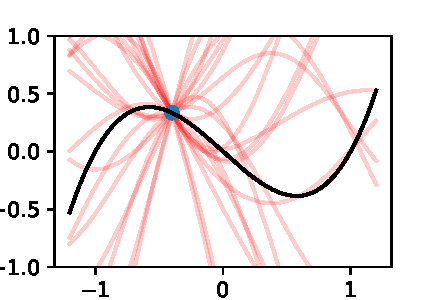
\includegraphics[width=\textwidth]{cub_GP_1_iters.pdf}
    %         \end{subfigure}%
    %         \begin{subfigure}[t]{0.4\textwidth}
    %             \centering
    %             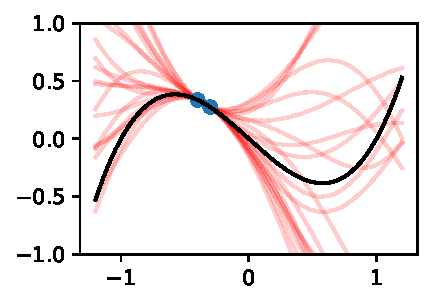
\includegraphics[width=\textwidth]{cub_GP_2_iters.pdf}
    %         \end{subfigure}
    %     \end{figure}}
\end{frame}

\begin{frame}
    \frametitle{Bayesian Acquisition Functions}
    \begin{itemize}
        \item $\mu(\bm{\theta}) := \E(D_\mathcal{GP}(\bm{\theta}))$ and
              $\mathrm{v}(\bm{\theta})
                  := \mathrm{Var}(D_\mathcal{GP}(\bm{\theta}))$
        \item Bayesian acquisition functions $A(\bm{\theta}),$ quantify how
              `desirable' it is to sample $\mathcal{D}(\bm{\theta})$ at
              $\bm{\theta}.$
        \item <2-> \cite{gutmann_bayesian_2016} minimise lower confidence bound
              $$
                  A_\text{LCB}(\bm\theta)
                  := \mu(\bm\theta) - \eta_t\sqrt{\mathrm{v}(\bm\theta)},
              $$
              the lower value of a confidence interval (determined by $\eta_t$).
              %   \begin{itemize}
              %       \item $\eta_t$ a slowly increasing function in $t,$ the
              %             number of previous samples
              %   \end{itemize}
              %   \item <3-> Expected improvement
              %   \begin{align*}
              %       A_\text{EI}(\bm\theta)
              %       := & \E[\max(\mu_\text{min} - \mathcal{D}_\mathcal{GP}(\bm\theta), 0)] % \\
              %       %   =  & (\mu_\text{min} - \mu(\bm\theta))
              %       %   \varPhi\left(\frac{\mu_\text{min} - \mu(\bm\theta)}{\sqrt{\mathrm{v}(\bm\theta)}}\right) \\
              %       %      & + \sqrt{\mathrm{v}(\bm\theta)}
              %       %   \phi\left(\frac{\mu_\text{min} - \mu(\bm\theta)}{\sqrt{\mathrm{v}(\bm\theta)}}\right)
              %   \end{align*}\begin{itemize}
              %       \item $\mu_\text{min} := \min_{\bm{\theta}} \mu(\bm\theta)$
              %             %   \item $\varPhi, \phi$ CDF and PDF of standard normal
              %   \end{itemize}
    \end{itemize}
\end{frame}

% \begin{frame}
%     \frametitle{Lower Confidence Bound example}
%     \begin{figure}
%         \centering
%         \begin{subfigure}[t]{0.4\textwidth}
%             \centering
%             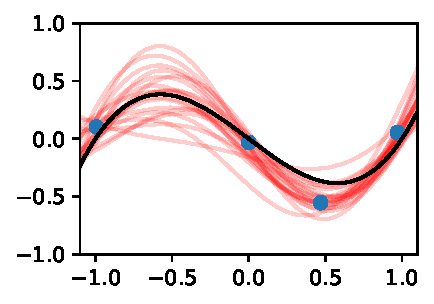
\includegraphics[width=\textwidth]{UCB_4_iters.pdf}
%         \end{subfigure}%
%         \begin{subfigure}[t]{0.4\textwidth}
%             \centering
%             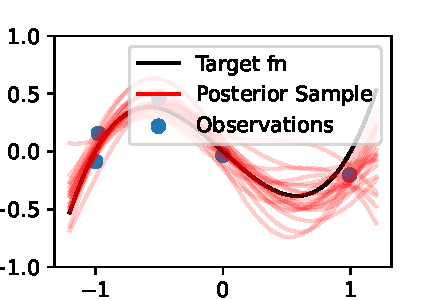
\includegraphics[width=\textwidth]{UCB_5_iters.pdf}
%         \end{subfigure}
%         \begin{subfigure}[t]{0.4\textwidth}
%             \centering
%             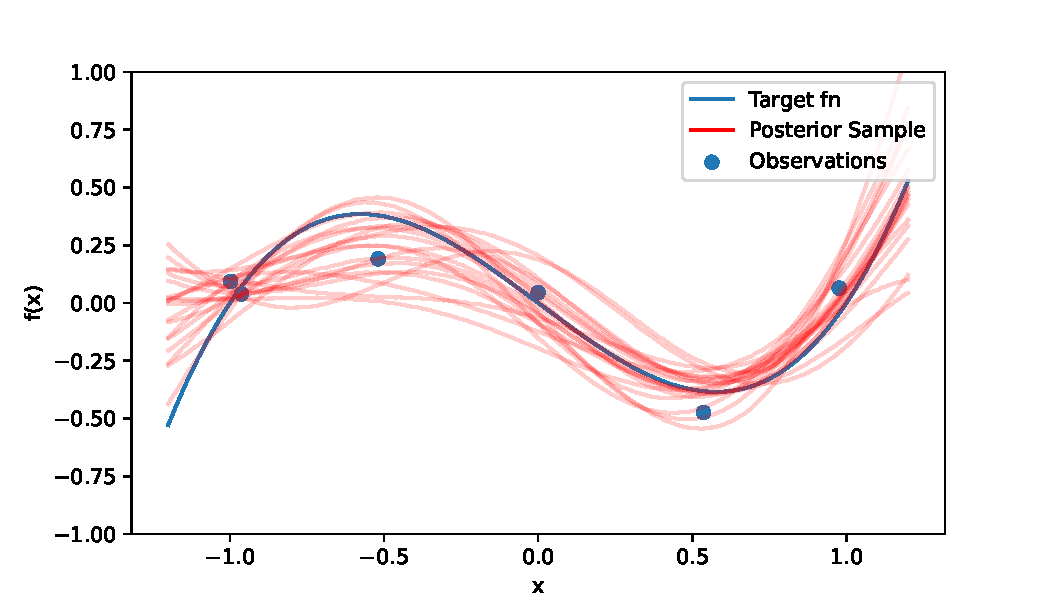
\includegraphics[width=\textwidth]{UCB_6_iters.pdf}
%         \end{subfigure}%
%         \begin{subfigure}[t]{0.4\textwidth}
%             \centering
%             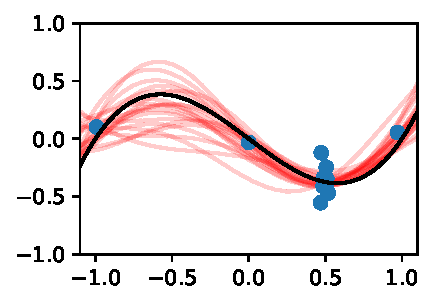
\includegraphics[width=\textwidth]{UCB_12_iters.pdf}
%         \end{subfigure}%
%     \end{figure}
% \end{frame}

\begin{frame}
    \frametitle{Vivax Model - Champagne et.\ al}
    \begin{figure}[htbp]
        \centering
        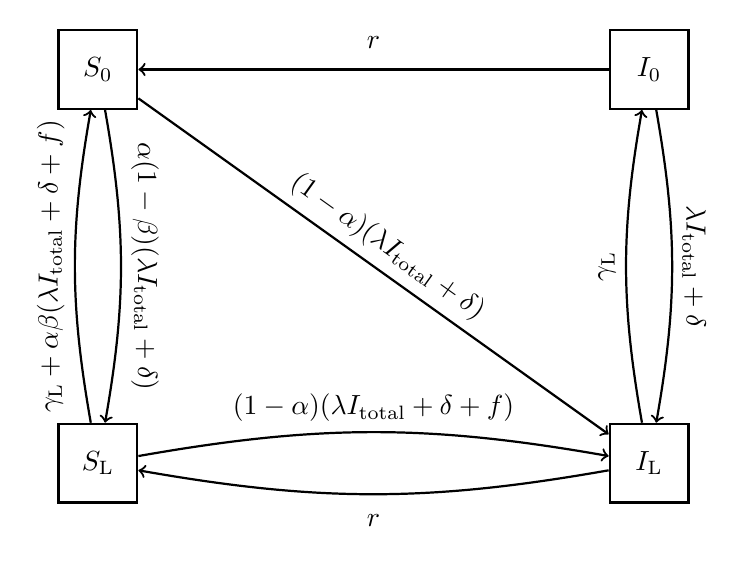
\begin{tikzpicture}[thick]
            \node[draw, minimum size=1cm] (S0) {$S_0$};
            \node[draw, right of=S0, minimum size=1cm, node distance=7cm] (I0)
            {$I_0$};
            \node[draw, below of=S0, minimum size=1cm, node distance=5cm] (SL)
            {$S_\mathrm{L}$};
            \node[draw, below of=I0, minimum size=1cm, node distance=5cm] (IL)
            {$I_\mathrm{L}$};
            \draw[->] (S0) edge[sloped] node[above]
                {$(1 - \alpha)(\lambda I_\mathrm{total} + \delta)$} (IL);
            \draw[->] (S0) edge[in = 80, out = 280, sloped] node[above]
                {$\alpha( 1 -\beta)(\lambda I_\mathrm{total} + \delta)$} (SL);
            \draw[->] (SL) edge[in = 260, out = 100, sloped] node [above]
                {$\gamma_\mathrm{L} + \alpha\beta(\lambda I_\mathrm{total} + \delta + f)$} (S0);
            \draw[->] (SL) edge[in = 170, out = 10, sloped] node [above]
                {$(1 - \alpha)(\lambda I_\mathrm{total} + \delta + f)$} (IL);
            \draw[->] (IL) edge[in = -10, out = 190] node [midway, label=below:
            {$r$}] (r) {} (SL);
            \draw[->] (IL) edge[in = 260, out = 100, sloped] node [above]
                {$\gamma_\mathrm{L}$} (I0);
            \draw[->] (I0) edge[in = 80, out = 280, sloped] node [above]
                {$\lambda I_\mathrm{total} + \delta$} (IL);
            \draw[->] (I0) edge node [midway, label=above:{$r$}] (r2) {} (S0);
        \end{tikzpicture}
        \caption{\cite{champagne_using_2022} \textit{P.\ vivax} model}
    \end{figure}
\end{frame}

\begin{frame}
    \frametitle{Champagne Model Parameters}\begin{itemize}
        \item $\alpha:$ proportion of those infected but cleared of blood stage
              infections
              (through treatment)
        \item $\beta:$ a further proportion that are also cleared of liver
              stage parasites,
              given that they were also cleared of blood stage infection
              (radical cure)
        \item $\lambda:$ the rate of infection
        \item $\gamma_L:$ rate of clearance of liver stage disease
        \item $f:$ rate of relapse
        \item $r:$ rate of blood stage clearance
    \end{itemize}
\end{frame}

% Simulated using the Doob-Gillespie algorithm, which is the standard way to
% get an exact simulation

\begin{frame}
    \frametitle{Model Simulation}
    \begin{figure}
        \centering
        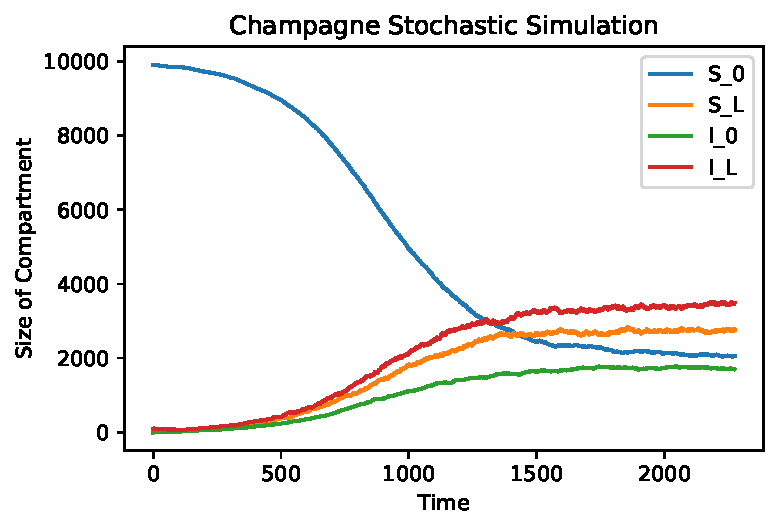
\includegraphics[width=0.8\textwidth]{
            ../../champagne_GP_images/champagne_simulation.pdf
        }
        \caption{
            Exact stochastic simulation using parameters reported in
            \cite{champagne_using_2022}. Population 10,000, initial infections 100.
        }
    \end{figure}
\end{frame}

\begin{frame}
    \frametitle{`Observed' Data}
    \begin{itemize}
        \item $\mathbf{Y}_\text{obs} := \{\iota_\text{obs}, \pi_\text{obs}, i_\text{obs}, p_{obs}\}$
              \begin{itemize}
                  \item $\iota_\text{obs}:$ weekly incidence around steady state equilibrium
                  \item $\pi_\text{obs}:$ prevalence around steady state equilibrium
                  \item $i_\text{obs}:$ incidence in the first month of the epidemic
                  \item $p_{obs}:$ prevalence after one month of simulation
              \end{itemize}
        \item <2-> $
                  \mathcal{D}(\alpha, \beta, \gamma_L, \lambda, f, r)$ is the
              $L_2$ norm of the relative differences
              $$
                  \sqrt{
                      \left(\frac{\iota - \iota_\text{obs}}{\iota_\text{obs}}\right)^2
                      + \left(\frac{\pi - \pi_\text{obs}}{\pi_\text{obs}}\right)^2
                      + \left(\frac{i - i_\text{obs}}{i_\text{obs}}\right)^2
                      + \left(\frac{p - p_\text{obs}}{p_\text{obs}}\right)^2
                  }
              $$
    \end{itemize}
\end{frame}

\begin{frame}
    \frametitle{GP choices}
    \begin{itemize}
        \item $\mathcal{GP}$ choices
              \begin{itemize}
                  \item Modelled $\ln\mathcal{D}$ as a Gaussian process
                  \item Matern kernel with $\nu = 5/2$
                  \item $\ell, \sigma^2_k, \sigma^2_o$ selected by leave
                        one out cross validation.
              \end{itemize}
    \end{itemize}
\end{frame}

\begin{frame}
    \frametitle{How did it go?}
    \only<2>{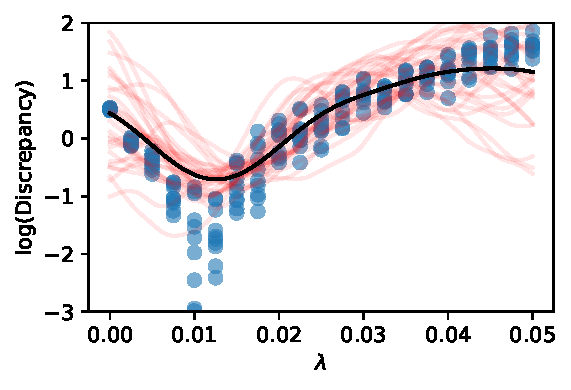
\includegraphics[width=\textwidth]{
            ../../champagne_GP_images/initial_lambda_slice_log_discrep.pdf}}
    \only<3>{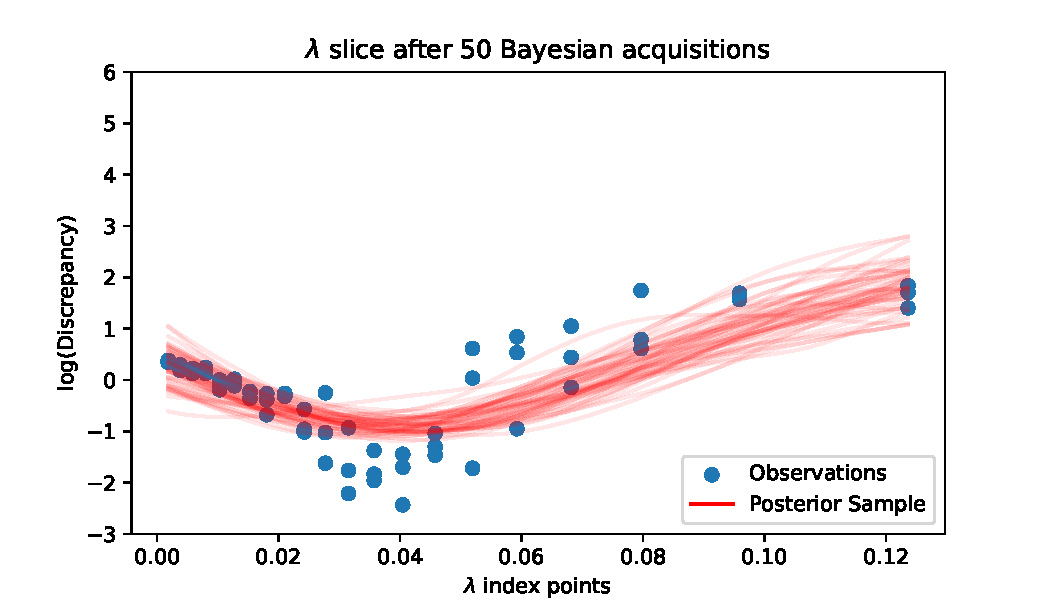
\includegraphics[width=\textwidth]{
            ../../champagne_GP_images/lambda_slice_50_bolfi_updates_log_discrep.pdf}}
    \only<4>{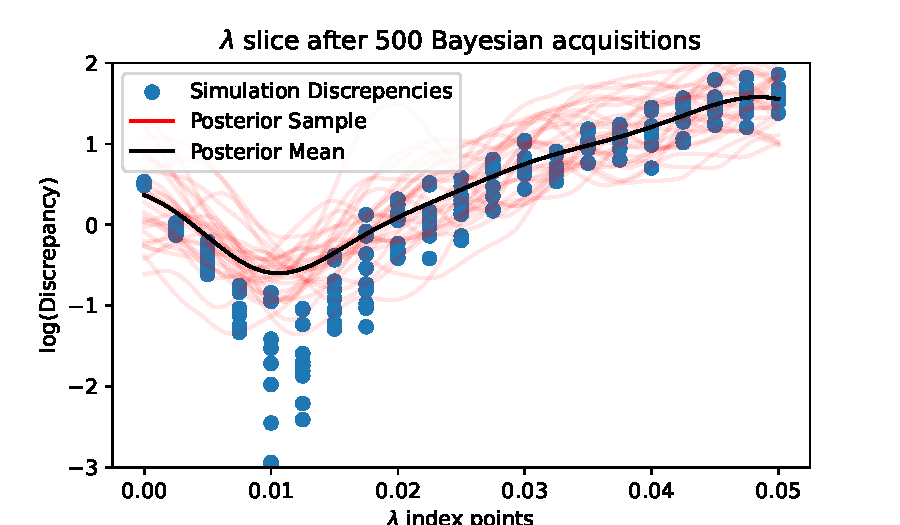
\includegraphics[width=\textwidth]{
            ../../champagne_GP_images/lambda_slice_500_bolfi_updates_log_discrep.pdf}}
    \only<5>{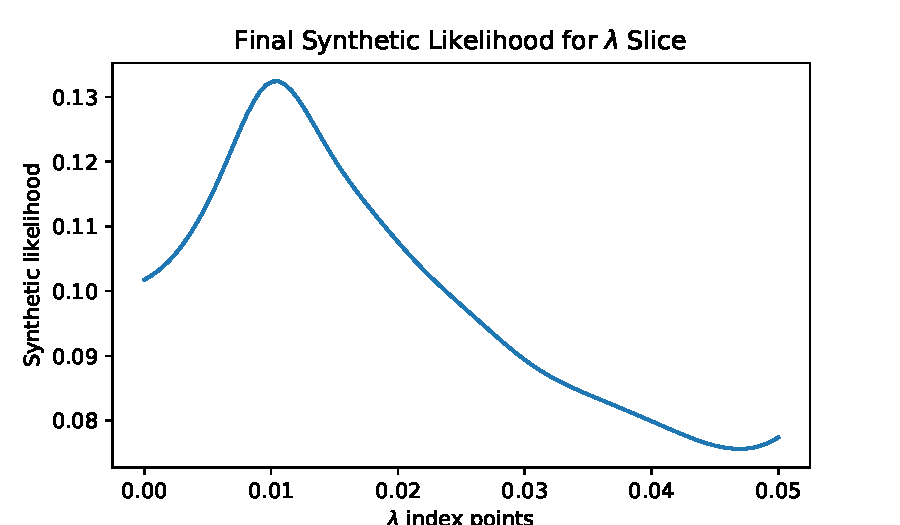
\includegraphics[width=\textwidth]{
            ../../champagne_GP_images/lambda_slice_500_synth_likelihood.pdf}}
    \only<6>{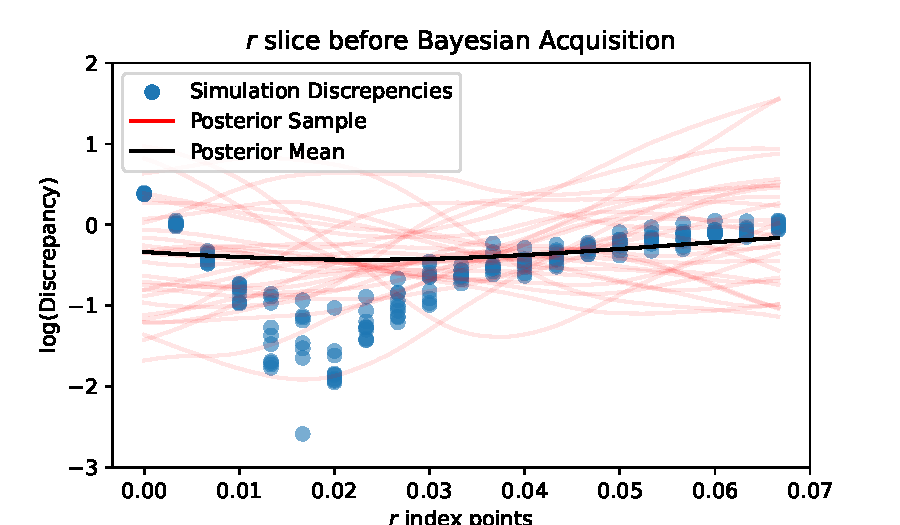
\includegraphics[width=\textwidth]{
            ../../champagne_GP_images/initial_r_slice_log_discrep.pdf}}
    \only<7>{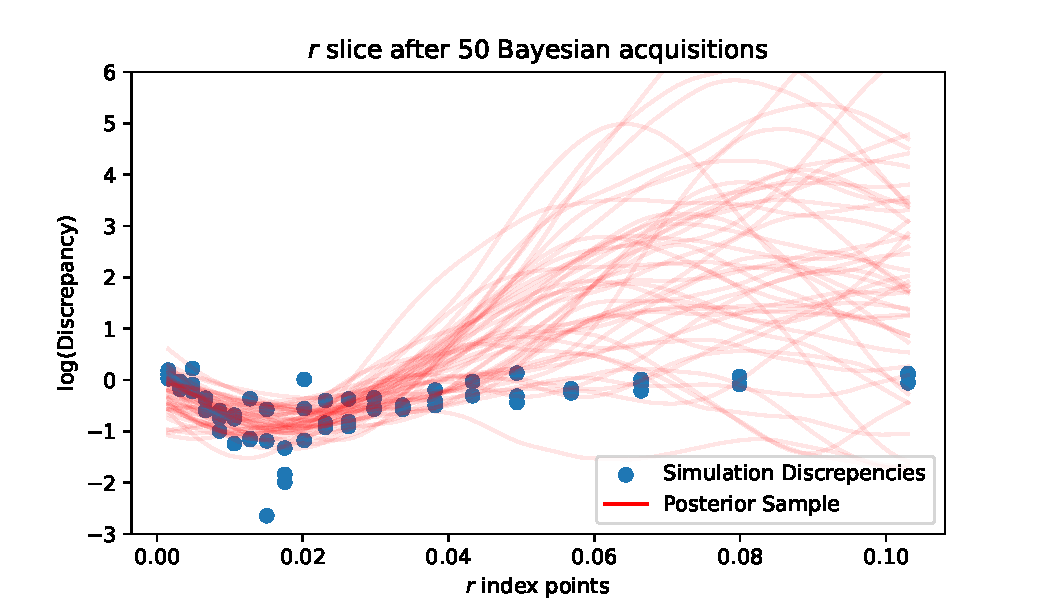
\includegraphics[width=\textwidth]{
            ../../champagne_GP_images/r_slice_50_bolfi_updates_log_discrep.pdf}}
    \only<8>{\includegraphics[width=\textwidth]{
            ../../champagne_GP_images/r_slice_500_bolfi_updates_log_discrep.pdf}}
    \only<9>{\includegraphics[width=\textwidth]{
            ../../champagne_GP_images/r_slice_500_synth_likelihood.pdf}}
\end{frame}

\begin{frame}
    \frametitle{Discussion}
    \begin{itemize}
        \item Bifurcation points effect:
              \begin{enumerate}
                  \item observation variance,
                  \item distribution of observations,
                  \item behaviour of the discrepency mean.
              \end{enumerate}
        \item Possible extensions:
              \begin{enumerate}
                  \item <2-> model $s^2(\bm{\theta})$,
                  \item <3-> choose a different distribution and moment match,
                  \item <4-> use a Student's $t-$process.
              \end{enumerate}
    \end{itemize}
\end{frame}

\begin{frame}
    \frametitle{Conclusion}
    \begin{itemize}
        \item Calibrating model parameters is important for scenario testing etc
        \item Successfully calibrated model parameters
        \item Could be used with more complicated models, even your model...
    \end{itemize}
\end{frame}

\begin{frame}
    \frametitle{Thanks to}
    \begin{itemize}
        \item Eamon Conway
        \item Jennifer Flegg
        \item Ivo Mueller
        \item Mueller lab and unimelb MMB group
    \end{itemize}
\end{frame}

\begin{frame}
    \frametitle{Bibliography}
    \printbibliography
\end{frame}

\end{document}